\normaltrue
\correctionfalse

%\UPSTIidClasse{12} % 11 sup, 12 spé
%\newcommand{\UPSTIidClasse}{12}

\exer{Poutre encastrée $\star$ \label{C2:10:Coh:526}}
\setcounter{numques}{0}
\UPSTIcompetence[2]{C2-10}
\index{Compétence C2-10}
\index{Torseur de cohésion}
\index{Diagramme des efforts intérieurs}

\begin{flushright}
\footnotesize{D'après documents Emmanuel PINAULT-BIGEARD.}
\end{flushright}


\ifcorrection
\else
\textbf{Pas de corrigé pour cet exercice.}
\fi

On donne la poutre encastrée suivante.

\begin{figure}[H]
\centering
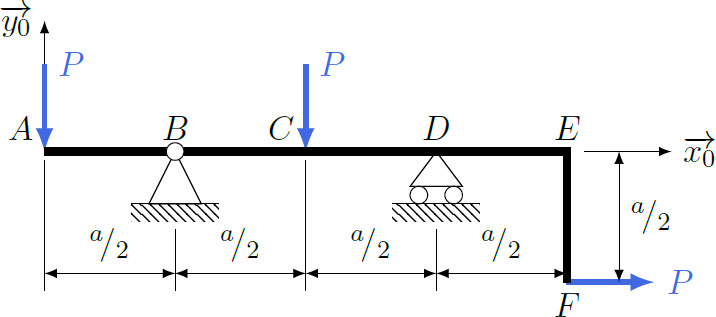
\includegraphics[width=\linewidth]{526_01}
%\caption{\label{61_01} Loi de commande de vitesse en trapèze}
\end{figure}


\question{Déterminer le torseur de cohésion.}
\ifprof
\else
\fi

\question{Identifier les sollicitations auxquelles est soumise la poutre.}
\ifprof
\else
\fi

\question{Tracer les diagrammes des efforts intérieurs.}
\ifprof
\else
\fi

\ifprof

\else
%\footnotesize
%\begin{enumerate}
%  \item $\left(fp + Mp^2\right) Z(p)=S_h P_h(p)-S_e P_e(p) - \dfrac{Mg}{p}$
%    \item $Q_e(p)=\left(S_a - S_b \right)pL(p) + \dfrac{V_t}{B_e} p P_e(p)$ et $mp^2 L(p) = -rL(p)+\left(S_a-S_b\right) P_e(t)-f'pL(p)$.
%\end{enumerate}
%\normalsize

\begin{flushright}
\footnotesize{Corrigé  voir \ref{C2:10:Coh:526}.}
\end{flushright}%
\fi